% !TEX root = saveliev_physics_general_course_1.tex
%!TEX TS-program = pdflatex
%!TEX encoding = UTF-8 Unicode


\chapter{ĐỘNG LỰC HỌC CỦA CHÁT ĐIỂM}\label{chap:2}

\section{Cơ học cổ điển. Phạm vi ứng dụng của nó}\label{sec:2_1}

Động học mô tả sự chuyển động của vật nhưng chưa đề cập tới vấn đề là tại sao vật lại chuyển động như thế này (chẳng hạn, chuyển động tròn đều hoặc thẳng nhanh dần đều) mà không như thế kia.

Động lực học nghiên cứu sự chuyển động của vật liên hệ với các nguyên nhân (các tương tác giữa các vật) gây ra một đặc trưng nào đó của chuyển động.

Ba định luật động lực học đã được Newton trình bày vào năm 1687 làm cơ sở của cơ học cổ điển hoặc cơ học Newton.

Các định luật Newton (cũng như tất cả các định luật vật lý còn lại) đã xuất hiện do sự khái quát hóa một số lượng lớn các sự kiện thực nghiệm. Sự đúng đắn của chúng (tuy đối với một phạm vi rất rộng lớn nhưng vẫn còn rất hạn chế của các hiện tưởng) được xác nhận bằng sự phù hợp giữa thí nghiệm với những kết luận rút ra từ những định luật đó.

Cơ học Newton đã đạt được nhiều thành tựu to lớn suốt trong hai thế kỷ, đến nỗi nhiều nhà vật lý của thế kỷ XIX đã tin vào sức mạnh toàn năng của nó. Người ta đã cho rằng giải thích một hiện tượng vật lý bất kỳ có nghĩa là đưa nó về một quá trình cơ học tuân theo các định luật Newton. Tuy nhiên với sự phát triển của khoa học người ta đã phát hiện ra các sự kiện mới không nằm trong phạm vi của cơ học cổ điển. Những sự kiện này đã được giải thích trong các thuyết mới là thuyết tương đối hẹp và cơ học lượng tử.

Trong thuyết tương đối hẹp, do Einstein xây dựng vào năm 1905, người ta đã xét lại tận gốc các quan niệm của Newton về không gian và thời gian. Sự xét lại này đã đưa tới việc xây dựng ``môn cơ học các vận tốc lớn'' hoặc như người ta gọi nó là cơ học tương đối tính. Tuy nhiên môn cơ học mới này không dẫn đến sự phủ nhận hoàn toàn môn cơ học Newton đã có. Các phương trình cơ học tương đối tính lại giới hạn (đối với các vận tốc nhỏ hơn vận tốc ánh sáng) đều chuyển thành các phương trình cơ học cổ điển. Như vậy, cơ học cổ đển đã nằm trong cơ học tương đối tính như một trường hợp riêng của nó và vẫn giữ nguyên tác dụng trước đây của nó đối với việc mô tả các chuyển động xảy ra với các vận tốc nhỏ.

Tình hình cũng tương tự đối với sự liên hệ giữa cơ học cổ điển và cơ học lượng tử ra đời tỏng những năm hai mươi của thế kỷ chúng ta do sự phát triển của vật lý nguyên tử. Các phương trình cơ học lượng tử tại giới hạn cũng cho (đối với các khối lượng lớn hơn khối lượng nguyên tử) các phương trình cơ học cổ điển. Do đó cơ học cổ điện cũng nằm trong cơ học lượng tử như là một trường hợp giới hạn của nó.

Như vậy, sự phát triển của khoa học đã không xóa bỏ cơ học cổ điển mà chỉ chứng tỏ sự ứng dụng hạn chế của nó. Cơ học cổ điện dựa trên các định luậ Newton là môn cơ học của các vật có các khối lượng lớn (so với khối lượng nguyên tử), chuyển động với các vận tốc nhỏ (so với vận tốc ánh sáng).

\section{Định luật Newton thứ nhất. Các hệ quy chiếu quán tính}\label{sec:2_2}

Định luật Newton thứ nhất được phát biểu như sau: \textit{mọi vật ở trạng thái nghỉ hay ở trạng thái chuyển động đều và thẳng chừng nào mà sự tác động từ phía các vật khác chưa buộc nó phải thay đổi trạng thái đó}. Cả hai trạng thái đã nêu đều có đặc điểm là gia tốc của vật bằng không. Do đó có thể diễn đạt định luậ thứ nhất dưới dạng sau đây: Vận tốc của một vật bất kỳ vẫn còn không đổi (trong trường hợp riêng, bằng không) cho đến lúc sự tác động từ phía các vật khác lên vật này gây ra sự biến đổi vận tốc đó.

Định luật Newton thứ nhất được nghiệm đúng không phải đối với mọi hệ quy chiếu. Ta đã để ý rằng đặc trưng của chuyển động phụ thuộc vào sự chọn hệ quy chiếu. Ta hãy xét hai hệ quy chiếu chuyển động với nhau với một gia tốc nào đó. Nếu vật đứng yên ododis với hệ quy chiếu này thì rõ ràng là nó sẽ chuyển động có gia tốc đối với hệ quy chế kia. Do đó, định luật Newton thứ nhất không thể được nghiêm đúng đồng thời trong cả hai hệ.

Hệ quy chiếu trong đó định luật Newton thú nhất được nghiệm đúng được gọi là \textbf{hệ quy chiếu quán tính}. Đôi khi người ta gọi chính định luật này là \textbf{định luật quán tính}. Hệ quy chiếu trong đó định luật Newton thứ nhất không được nghiệm đúng được gọi là hệ quy chiếu không quán tính. Có vô số các hệ quy chiếu quán tính. Một hệ quy chiếu bất kỳ chuyển động thẳng và đều (tức là với vận tốc không đổi) đối với một hệ quy chiếu quán tính nào đó cũng sẽ là một hệ quy chiếu quán tính. Chi tiết hơn về điều này sẽ nói ở \ref{sec:2_7}.

Bằng thực nghiệm đã thiết lập rằng một hệ quy chiếu mà tâm trùng với Mặt trời còn các trục hướng về các ngôi sao đã được chọn một cách thích hợp là một hệ quy chiếu quán tính. Hệ này được gọi là \textbf{hệ quy chiếu nhật tâm}. Một hệ quy chiếu bất kỳ chuyển động đều và thẳng đối với hệ nhật tâm sẽ là một hệ quy chiếu quán tính.

Trái đất chuyển động đối với Mặt trời và các ngôi sao theo một quỹ đạo cong có dạng đường elip. Chuyển động cong luôn luôn xảy ra với một gia tốc nào đó. Ngoài ra, Trái đất quay xung quanh trục của nó. Theo các nguyên nhân này, hệ quy chiếu gắn với mặt đất sẽ chuyển động có gia tốc đối với hệ quy chiếu nhật tâm và không là hệ quy chiếu quán tính. Tuy vậy gia tốc của hệ đó là nhỏ đến nỗi trong một số lớn trường hợp, thực tế có thể coi nó là hệ quy chiếu quán tính. Nhưng đôi khi tính chất không quán tính của hệ quy chiếu gắn với Trái đất có ảnh hưởng lớn tới đặc tính của các hiện tượng cơ học được xét so với nó. Sau nay ta sẽ khảo sát một số trường hợp như vậy.

\section{Khối lượng và xung lượng của vật}\label{sec:2_3}

Tác động lên vật đã cho từ phía các vật khác làm biến đổi vận tốc của nó, tức là truyền cho vật đã cho một gia tốc. Thí nghiệm chứng tỏ rằng cùng một tác động như nhau truyền cho những vật khác nhau những gia tốc khác nhau về độ lớn. Mọi vật đều chống lại những xu hướng làm biến đổi trạng thái chuyển động của nó. Tính chất này của các vật được gọi là \textbf{quán tính}. Để miêu tả định lượng tính chất của quán tính nguời ta dùng đại lượng gọi là \textbf{khối lượng} của vật.

Để xác định khối lượng của một vật nào đó cần phải so sánh nó với khối lượng của vật được thừa nhận làm mẫu của khối lượng. Cũng có thể so sánh khối lượng của vật đã cho với khối lượng của một vật nào đó có khối lượng đã biết (được xác định bằng cách so sánh với mẫu). Có thể thực hiện phép so sánh các khối lượng $m_1$ và $m_2$ của hai chất điểm (hạt) bằng cách sau. Ta hãy đặt các hạt này trong những điều kiện mà có thể bỏ qua sự tương tác của chúng với các vật khác. Hệ các vật chỉ tương tác giữa chúng với nhau mà không tương tác với các vật khác được gọi là \textbf{hệ kính}. Do đó ta nghiên cứu hệ kín gồm hai hạt. Nếu bắt các hạt này tương tác với nhau (chẳng hạn, va chạm trực tiếp với nhau), thì các vận tốc của chúng nhận các số gia $\Delta\vec{v}_1$ và $\Delta\vec{v}_2$. Thí nghiệm cho thấy các số gia này luôn luôn có các hướng ngược nhau, tức là khác nhau về dấu. Ngay cả tỷ số module của số gia các vận tốc cũng không phụ thuộc vào cách và cường độ tương tác của hai vật đã cho\footnote{Điều này đúng trong trường hợp khi vận tốc ban đầu và vận tốc cuối của các hạt nhỏ hơn vận tốc ánh sáng $c$.}. Tỷ số này được lấy bằng nghịch đảo của tỷ số các khối lượng của các vật được xét:
\begin{equation}\label{eq:2_1}
\frac{|\Delta\vec{v}_1|}{\Delta\vec{v}_2} = \frac{m_2}{m_1}
\end{equation}

\noindent
(vật có quán tính lớn hơn, nghĩa là vật có khối lượng lớn hơn bị thay đổi vận tốc ít hơn). Nếu để ý tới hướng tương đối của các vecor $\Delta\vec{v}_1$ và $\Delta\vec{v}_2$, thì có thể viết hệ thức \eqn{2_1} dưới dạng
\begin{equation}\label{eq:2_2}
m_1 \Delta\vec{v}_1 = - m_2 \Delta\vec{v}_2.
\end{equation}

Trong cơ học Newton (tức là môn cơ học mà các định luật Newton là nền tảng của nó) khối lượng của vật được giả thiết là một đại lượng không đổi, không phụ thuộc vào vận tốc của vật. Với các vận tốc nhỏ hơn vận tốc ánh sáng $c$ (với $v\ll c$) giả thuyết này thực tế được nghiệm đúng. Lợi dụng sự không đổi của khối lượng, ta hãy biểu diễn đẳng thức \eqn{2_2} như sau:
\begin{equation}\label{eq:2_3}
\Delta(m_1 \vec{v}_1) = - \Delta(m_2 \vec{v}_2).
\end{equation}

Tích của khối lượng của vật với vận tốc của nó được gọi là \textbf{xung lượng của vật}. Nếu ký hiệu xung lượng bằng chữ $\vec{p}$, ta có
\begin{equation}\label{eq:2_4}
\vec{p} = m \vec{v}.
\end{equation}

\noindent
Định nghĩa \eqref{eq:2_4} là đúng đối với các chất điểm (các hạt) và các vật lớn chuyển động tịnh tiến. Trong trường hợp một vật lớn chuyển động không tịnh tiến, cần phải quan niệm vật như một tập hợp các chất điểm có các khối lượng $\Delta m_i$, xác định các xung lượng $\Delta m_i\vec{v}_i$ của các chất điểm này và sau đó cộng các xung lượng này lại theo vector. Kết quả là người ta được xung lượng toàn phần của vật:
\begin{equation}\label{eq:2_5}
\vec{p} = \sum_{i} m_i \vec{v}_i.
\end{equation}

\noindent
Trong chuyển động tịnh tiến của vật tất cả các $\vec{v}_i$ là như nhau và công thức \eqn{2_5} chuyển thành \eqref{eq:2_4}.

Nếu thay vào \eqn{2_3} các tích $m\vec{v}$ bằng các xung lượng $\vec{p}$, ta đi tới hệ thức $\Delta\vec{p}_1=\Delta\vec{p}_2$, từ đó $\Delta(\vec{p}_1+\vec{p}_2)=0$. Sự bằng không của số gia của một đại lượng có nghĩa chính đại lượng này là không đổi. Như vậy, ta đi tới kết luận là \textit{xung lượng toàn phần của một hệ kín gồm hai hạt tương tác với nhau là không đổi}:
\begin{equation}\label{eq:2_6}
\vec{p} = \vec{p}_1 + \vec{p}_2 = \text{constant}.
\end{equation}

\noindent
Điều khẳng định đưa ra ở trên là nội dung của \textbf{định luật bảo toàn xung lượng}. Trong \ref{sec:3_10} ta sẽ nghiên cứu định luật này một cách chi tiết hơn.

Ta hãy để ý rằng trong cơ học tương đối tính (xem chương \ref{chap:8}) biểu thức cho xung lượng có dạng phức tạp hơn \eqn{2_4}:
\begin{equation}\label{eq:2_7}
\vec{p} = \frac{m \vec{v}}{\sqrt{1 - v^2/c^2}}.
\end{equation}

\noindent
Ở đây $m$ được gọi là \textbf{khối lượng tĩnh} của vật (khối lượng của vật khi $v=0$), $c$ là vận tốc ánh sáng trong chân không. Có thể giải thích biểu thức \eqref{eq:2_7} để sao cho khối lượng của vật không còn không đổi (như được giả thiết trong cơ học Newton) mà biến đổi với vận tốc theo định luật
\begin{equation}\label{eq:2_8}
m(v) = \frac{m}{\sqrt{1 - v^2/c^2}}
\end{equation}

\noindent
Khi đó có thể biểu diễn biểu thức \eqn{2_7} dưới dạng
\begin{equation}\label{eq:2_9}
\vec{p} = m(v)\,\vec{v}
\end{equation}

\noindent
tương tự như biểu thức \eqn{2_4}.

Khối lượng $m(v)$ xác đình bằng công thức \eqn{2_8} được gọi là \textbf{khối lượng tương đối tính} hay \textbf{khối lượng động}. Dưới đây ta sẽ ký hiệu nó bằng $\mr$.

\section{Định luật Newton thứ hai}\label{sec:2_4}

Định luật Newton thứ hai nói rằng, \textit{tốc độ biến thiên xung lượng của vật bằng lực $\vec{F}$ tác dụng lên vật}:
\begin{equation}\label{eq:2_10}
\diff{\vec{p}}{t} = \vec{F}.
\end{equation}

\noindent
Phương trình \eqref{eq:2_10} được gọi là \textbf{phương trình chuyển động của vật}.

Theo \eqn{2_4} nếu thay $\vec{p}$ bằng tích $m\vec{v}$, và chuys rằng trong cơ học Newton khối lượng được giả thiết là không đổi, thì có thể biểu diễn hệ thức \eqn{2_10} dưới dạng
\begin{equation}\label{eq:2_11}
m\vec{a} = \vec{F}
\end{equation}

\noindent
trong $\vec{a}=\dot{\vec{v}}$. Như vậy ta đã đi tới một cách diễn đạt khác của định luật Newton thứ hai: \textit{tích khối lượng của vật với gia tốc của nó bằng lực tác dụng lên vật}.

Hệ thức \eqref{eq:2_11} đã gây ra và còn tiếp tục gây ra nhiều sự tranh cãi giữa các nhà vật lý. Cho đến nay vẫn chưa có một sự giải thích được mọi người thừa nhận về hệ thức này. Điều phức tạp là ở chỗ không tồn tại các cách độ lập để xác định các đại lượng $m$ và $\vec{F}$ tham gia vào \eqn{2_11}. Để xác định một trong các đại lượng ($m$ hay $\vec{F}$), cần phải sử dụng hệ thức \eqn{2_11} liên hệ đại lượng này với đại lượng kia và với gia tốc $\vec{a}$. For example, according to S. Khaikin\footnote{S. E. Khaikin. Fizicheskie osnovy mekhaniki (The Physical Fundamentals of Mechanics). Moscow, Fizmatgiz (1963), p. 104.}, ``Vì để thiết lập cách đo khối lượng của vật người ta sử dụng ngay chính định luật Newton hai (độ lớn của khối lượng của vật được xác định bằng cách đo đồng thời lực và gia tốc), cho nên định luật Newton thứ hai một mặt khẳng định rằng gia tốc tỷ lệ với lực, còn mặt khác xác định khối lượng của vật như các tỷ số của lực tác dụng lên vật với gia tốc do lực này truyền cho''.

R. Feynman vin vào ý nghĩa của luật Newton thứ hai đã nói như sau: ``Ta hãy hỏi ngay rằng: ý nghĩa của công thức $F=ma$ là gì? Ta hiểu một cách trực giác khối lượng là gì; ta cũng có thể xác định được gia tốc nếu ta hiểu vị trí là gì và thời gian là gì. Do đó chúng ta sẽ không tranh luận về ý nghĩa của các khái niệm này mà ta tập trung vào khái niệm mới về lực. Và ở đây câu trả lời cũng rất đơn giản: nếu vật được gia tốc có nghĩa là có lực tác dụng lên nó. Các định luật Newton đã nói như vậy và một định nghĩa chính xác nhất và đẹp nhất trong các định nghĩa có thể được của lực là, lực là khối lượng của vật nhân với gia tốc của nó\ldots''. Tuy nhiên ``\ldots khi khám phá ra định luật cơ bản, định luật đó khẳng định rằng lực là khối lượng nhân với gia tốc, và sau đó định nghĩa lực là tích của khối lượng với gia tốc thì chúng ta không tìm thấy một điều gì mới nữa\ldots những ý kiến như vật không thể tạo nên nội dung cả môn vật lý: vì sao ta đưa ra các định nghĩa luẩn quẩn về lực\ldots không bao giờ và không một ai đã rút ra một điều gì từ một định nghĩa\ldots. Nội dung thực của các định luật Newton là như sau: phải bổ sung cho định luật $\vec{F}=m\vec{a}$ giả thiết rằng lực có các tính chất độc lập; nhưng chưa một ai, kể cả Newton, mô tả đầy đủ các tính đặc trưng độc lập của các lực\ldots''\footnote{R. P. Feynman, R. B. Leighton, M. Sands. The Feynman Lectures on Physics. Reading, Mass., Addison-Wesley (1965), p. 12-1.}.

Ta hãy nhấn mạnh rằng định luật Newton thứ hai (cũng như cả hai định luật kia) là định luật thực nghiệm. Nó được ra đời do sự khái quát hóa các thí nghiệm và quan sát nhất định.

Trong trường hợp riêng, khi $\vec{F}=0$ (tức là khi không có tác động lên vật từ phía các vật kkhasc) gia tốc suy ra từ \eqn{2_11} cũng bằng không. Kết luận này trùng với điều khẳng định của định luật Newton thứ nhất. Do đó định luật thứ nhất được chứa trong định luật thứ hai như một trường hợp riêng của nó. Mặc dù vậy, định luật thứ nhất được trình bày một cách độc lập với định luật thứ hai vì trong đó thực ra chứa đựng một tiên đề (một điều khẳng định) về sự tồn tại của các hệ quy chiếu quán tính.

Để kết luận ta hãy chú ý rằng khi chọn một cách độc lập các đơn vị của khối lượng, của lực và của gia tốc, cần phải viết biểu thúc của định luật thứ hai dưới dạng
\begin{equation}\label{eq:2_12}
m\vec{a} = k\vec{F}
\end{equation}

\noindent
trong đó $k$ là hệ số tỷ lệ.

\section{Đơn vị và thứ nguyên của các đại lượng vật lý}\label{sec:2_5}

Các định luật của vật lý, như đã nhận xét, đều thiết lập các hệ thức định lượng giữa các đại lượng vật lý. Để thiết lập các hệ thức như thế cần phải có khả năng đo đạc các đại lượng vật lý khác nhau.

Đo một đại lượng vật lý nào đó (chẳng hạn vận tốc) có nghĩa là so sánh nó với một đại lượng cùng dạng (trong ví dụ đã nêu là vận tốc) được thừa nhạn làm đơn vị.

Nói chung, đối với mỗi đại lượng vật lý đã có thể thiết lập đơn vị của nó một cách tùy ý, không phụ thuộc vào các đại lượng khác. Tuy nhiên dường như là, về nguyên tắc, có thể bằng lòng với việc chọn tùy tiện các đơn vị đối với một số đại lượng bất kỳ (tối thiểu là ba) được thừa nhận làm các đơn vị cơ bản. Với mục đích đó có thể thiết lập các đơn vị của tất cả các đại lượng khác nhờ các đơn vị cơ bản bằng cách đã sử dụng các định luật vật lý liên hệ một đại lượng tương ứng với các đại lượng cơ bản hoặc với các đại lượng mà các đơn vị của chúng cũng đã được thiết lập bằng cách tương tự.

Ta hãy làm sáng tỏ điều vừa nói bằng ví dụ sau. Giả sử rằng ta đã thiết lập được các đơn vị cho khối lượng và gia tốc. Hệ thức \eqref{eq:2_12} liên hệ một cách có quy luật các đại lượng này với đại lượng vật lý thứ ba là lực. Ta hãy chọn đơn vị của lực sao cho hệ số tỷ lệ trong phương trình này bằng đơn vị. Khi đó công thức \eqref{eq:2_12} có dạng đơn giản hơn:
\begin{equation}\label{eq:2_13}
m\vec{a} = \vec{F}.
\end{equation}

\noindent
Từ \eqn{2_13} suy ra rằng đơn vị đã thiết lập của lực là một lực mà dưới tác dụng của nó, vật với khối lượng bằng đơn vị sẽ có gia tốc cũng bằng đơn vị [thay thế vào \eqn{2_13} $F=1$ và $m=1$ sẽ cho $a=1$].

Với cách chọn các đơn vị đã nêu, các hệ thức vật lý có dạng đơn giản hơn. Ngay bản thân tập hợp các đơn vị cũng tạo thành một hệ xác định.

Tồn tại một số hệ không giống nhau do cách chọn các đơn vị cơ bản. Các hệ mà các đơn vị độ dài, khối lượng và thời gian là cơ sở cho nó được gọi là các \textbf{hệ tuyệt đối}.

Ở Liên Xô, từ ngày 1 tháng giêng năm 1963 người ta đưa ra tiêu chuẩn quốc gia GOST 9867-61, nó quy định việc sử dụng bệ đơn vị quốc tế, ký hiệu là SI. Hệ đơn vị này phải được sử dụng tốt nhất vào tất cả các lĩnh vực khoa học, kỹ thuật và kinh tế quốc dân, cũng như trong giảng dạy. Các đơn vị cơ bản của SI là: đơn vị độ dài là met (ký hiệu là \si{\metre}), đơn vị khối lượng là kiloram (\si{\kilo\gram}) và đơn vị thời gian là giây (\si{\second}). Như vậy, SI thuộc về số các hệ tuyệt đối. Ngoài ba đơn vị đã nêu, để làm các đơn vị cơ bản, hệ SI còn có đơn vị cường độ dòng diện là ampe (\si{\ampere}), đơn vị nhiệt độ nhiệt động học là kelvin (\si{\kelvin}), đơn vị cường độ ánh sáng là candela (\si{\candela}) và đơn vị lượng chất là mol (\si{\mole}). Về các đơn vị này ta sẽ nói trong những phần tương ứng của giáo trình.

Met được định nghĩa là một độ dài bằng $1,650,763.73$ bước sóng trong chân không của bức xạ ứng với sự chuyển giữa các mức \enlevel{2}{p}{10} và \enlevel{5}{d}{5} của nguyên tử krypton-86\footnote{Ý nghĩa của các ký hiệu này sẽ được giải thích trong phần ``Vật lý nguyên tử''.} (vạch mày da cam krypton-86). Met gần bằng $1/40,000,000$ phần độ dài của kinh tuyến Trái đất. Người ta cũng dùng các bội và ước của đơn vị này: kilomet ($\SI{1}{\kilo\metre}=\SI{103}{\metre}$), centimet ($\SI{1}{\centi\metre}=\SI{e-2}{\metre}$), milimet ($\SI{1}{\milli\metre}=\SI{e-3}{\metre}$), micromet ($\SI{1}{\micro\metre}=\SI{e-6}{\metre}$),v.v...

Kilogam là khối lượng của một vật bằng platin-iridi\footnote{Hợp kim platin với iridi có độ cứng lớn và độ bền chống bị ăn mòn (nghĩa là ít chịu tác dụng hóa học của môi trường xung quanh).} được giữ ở Phòng Cân đo Quốc tế tại S\`evre (gần Paris). Vật này được gọi là nguyên mẫu quốc tế của kilogram. Khối lượng mẫu gần bằng khối lượng của $\SI{1000}{cm^3}$ nước nguyên chất ở $\SI{4}{^{\circ}C}$. Một gam bằng $1/1000$ kilogam.

Giây được định nghĩa là khoảng thời gian bằng tổng của $9192631770$ chu kỳ bức xạ ứng với sự chuyển giữa hai mức trạng thái cơ bản siêu mỏng của nguyên tử cesium-133. Giây gần bằng $1/86400$ ngày mặt trời trung bình.

Trong vật lý người ta cũng dùng hệ đơn vị tuyệt đối gọi là hệ CGS. Các đơn vị cơ bản của hệ này là centimet, gam và giây.

Các đơn vị của các đại lượng mà ta đưa vào trong động học (vận tốc và gia tốc) là các đơn vị dẫn xuất từ các đơn vị cơ bản. Như vậy, vận tốc của một vật chuyển động đều đi được một quãng đường bằng một đơn vị độ dài (met ha centimet) trong một đơn vị thời gian (giây) được lấy làm đơn vị vận tốc.. Đơn vị này được ký hiệu bằng \si{\metre\per\second} trong hệ SI và \si{\centi\metre\per\second} trong hệ CGS. Gia tốc của một chuyển động biến đổi đều mà trong đó vận tốc của vật trong một đơn vị thời gian (giây) bị biến đổi một đơn vị (\si{\metre\per\second} hay \si{\centi\metre\per\second}) được lấy làm đơn vị gia tốc. Đơn vị này đucợ ký hiệu là \si{\metre\per\square\second} trong hệ SI và \si{\centi\metre\per\square\second} trong hệ CGS.

Đơn vị lực trong SI được gọi là newton (\si{\newton}). Theo \eqref{eq:2_13}, một newton bằng lực mà dưới tác dụng của nó một vật có khối lượng \SI{1}{\kilo\gram} có được một gia tốc \SI{1}{\metre\per\square\second}. Đơn vị lực trong hệ CGS được gọi là dyne (\si{\dyne}). Một dyne bằng lực mà dưới tác dụng của nó một vật có khối lượng \SI{1}{\gram} có được gia tốc \SI{1}{\centi\metre\per\square\second}. Giữa newton và dyne có hệ thức sau:
\begin{equation*}
\SI{1}{\newton} = \SI{1}{\kilo\gram} \times \SI{1}{\metre\square\second} = \SI{e3}{\gram} \times \SI{e2}{\centi\metre\square\second}
\end{equation*}

Trong kỹ thuật người ta sử dụng rộng rãi hệ MkGS (thường được gọi là hệ đơn vị kỹ thuật). Các đơn vị cơ bản của hệ này là mét, kilogam lực (kgf) và giây. Kilogam lực được định nghĩa la lực truyền cho khối lượng 1kg một gia tốc bằng $\SI{9.80655}{\metre\per\second}$. Từ định nghĩa này suy ra rằng $\SI{1}{\kgf}=\SI{9.80655}{\newton}$ (gần đúng \SI{9.81}{\newton}).

Theo \eqn{2_13} khối lượng của một vật mà dưới tác dụng của lực là 1kgf, vật có gia tốc \SI{1}{\metre\per\square\second} phải được lấy làm đơn vị khối lượng trong hệ MkGS. Đơn vị này được ký hiệu là {\kgf\second\squared\per\metre}, nó không có tên gọi đặc biệt \footnote{See L. A. Sena. Units of Physical Quantities and Their Dimensions. 2nd ed., Moscow, Mir Publishers (1975), pp. 9, 54}, none of them has been legalized, and it is designated \si{\kgf\second\squared\per\metre}. Rõ ràng $\SI{1}{\kgf\second\squared\per\metre}=\SI{9.80655}{\kilo\gram}$ (gần đúng là \SI{9.81}{\kilo\gram}).
Từ cách xây dựng các hệ đơn vị suy ra rằng sự thay đổi các đơn vị cơ bản kéo theo sự thay đổi các đơn vị dẫn xuất. Chẳng hạn, nếu lấy phút làm đơn vị thơi gian thay cho giây, tức là tăng đơn vị thời gian lên $60$ lần thì đơn vị gia tốc giảm $3600$ lần.

Hệ thức chỉ ra đơn vị của một đại lượng nào đó sẽ biến đổi như thế nào khi biến đổi các đơn vị cơ bản được gọi là thú nguyên của đại lượng này. Để ký hiệu thứ nguyên của một đại lượng vật lý tùy ý người ta dùng ký hiệu bằng chữ của nó đặt trong các dấu ngoặc vuông. Chẳng hạn, ký hiệu $[v]$ có nghĩa là thứ nguyên của vận tốc. Đối với thứ nguyên của các đại lượng cơ bản người ta dùng các ký hiệu đặc biệt: đối với độ dài là $l$, khối lượng là $m$ và thời gian là $t$, có thể viết:
\begin{equation*}
[l] = \text{L},\quad [m] = \text{M},\quad [t] = \text{T}.
\end{equation*}

Trong các ký hiệu đã nêu thứ nguyên của một đại lượng vật lý tùy ý có dạng L$^{\alpha}$M$^{\beta}$T$^{\gamma}$ ($\alpha$, $\beta$ và $\gamma$ có thể là dương cũng như âm, trong trường hợp riêng, chúng có thể bằng không). Các viết này có ý nghĩa là khi tăng đơn vị độ dài lên $n_1$ lần thì đơn vị của đại lượng đã cho sẽ tăng $n_1^{\alpha}$ lần (một cách tương ứng, con số biểu thị giá trị của đại lượng theo các đơn vị này sẽ giảm $n_1^{\alpha}$ lần). Khi tăng đơn vị khối lượng lên $n_2$ lần, đơn vị của đại lượng đã cho tăng $n_2^{\beta}$ lần, và cuối cùng khi tăng đơn vị thời gian lên $n_3$ lần thì đơn vị của đại lượng đã cho tăng $n_3^{\gamma}$ lần.

Vì các định luật vật lý không thể phụ thuộc vào sự chọn các đơn vị của các đại lượng có mặt trong chúng, nên các thứ nguyên của cả hai vế của phương trình biểu diễn các định luật này phải giống nhau. Điều kiện này có thể được sử dụng, đầu tiên là để kiểm tra sự đúng đắn của các hệ thúc vật lý thu được và thú hai là để thiết lập các thứ nguyên của các đại lượng vật lý. Chẳng hạn, vận tốc được định nghĩa là $v = \Delta s/\Delta t$. Thứ nguyên của $\Delta s$ bằng L, thứ nguyên của $\Delta t$ bằng T. Thứ nguyên của vế phải của hệ thức đã viết bằng $[\Delta s]/[\Delta t]=\text{L/T}=\text{LT}^{-1}$. Thứ nguyên của vế trái cũng phải là như vậy. Do đó,
\begin{equation}\label{eq:2_14}
[v] = \text{LT}^{-1}.
\end{equation}

\noindent
Hệ thức đã viết được gọi là công thức thứ nguyên, còn vế phải của nó là thứ nguyên của đại lượng tương ứng (trong trường hợp đã cho là vận tốc).

Dạ vào hệ thức $a = \Delta v/\Delta t$ có thể thiết lập thú nguyên của gia tốc:
\begin{equation}\label{eq:2_15}
[a] = \frac{[\Delta v]}{[\Delta t]} = \frac{\text{LT}^{-1}}{\text{T}} = \text{LT}^{-2}.
\end{equation}

\noindent
Thứ nguyên của lực
\begin{equation}\label{eq:2_16}
[F] = [m][a] = \text{MLT}^{-2}.
\end{equation}

\noindent
Các thứ nguyên của tất cả các đại lượng khác cũng được thiết lập một cách tương tự.

\section{Định luật Newton thứ ba}\label{sec:2_6}

Mọi tác dụng của các vật với nhau mang đặc trưng của tác dụng tương hỗ: nếu vật $1$ tác dụng lên vật $2$ một lực $\vec{F}_{21}$ thì vật $2$ đến lượt mình lại tác dụng lên vật $1$ một lực $\vec{F}_{12}$.

\begin{figure}[!htb]
	\begin{center}
		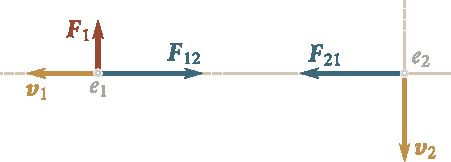
\includegraphics[scale=1]{figures/ch_02/fig_2_1.pdf}
		\caption[]{}
		\label{fig:2_1}
	\end{center}
\end{figure}

Định luật Newton thứ ba khẳng định rằng \textit{các lực mà các vật có tương tác tác dụng lẫn nhau sẽ bằng nhau về độ lớn và ngược chiều nhau}. Dùng các ký hiệu đã nêu ở trên về các lực, nội dung của định luật thứ ba có thể biểu diễn dưới dạng đẳng thức:
\begin{equation}\label{eq:2_17}
\vec{F}_{12} = - \vec{F}_{21}.
\end{equation}

Từ định luật Newton thứ ba suy ra rằng các lực xuất hiện từng cặp: có thể so sánh một lực bất kỳ đặt vào một vật nào đó với một lực bằng nó về độ lớn và ngược chiều đặt vào một vật khác tương tác với vật đã cho.

Định luật Newton thứ ba không phải bao giờ cũng đúng, Nó được nghiệm đúng một cách hoàn toàn nghiêm ngặt trong trường hợp các tương tác tiếp xúc (tức là các tương tác được quan sát khi các vật tiếp xúc trực tiếp) cũng như khi các tương tác của các vật đứng yen nằm cách nhau một khoảng nào đó.

Để làm ví dụ về sự vi phạm định luật Newton thứ ba, có thể dùng một hệ gòm hai hạt mang điện $e_1$ và $e_2$ chuyển động trong lúc khảo sát, như đã chỉ trên \fig{2_1}. Trong điện động lực học người ta đã chứng minh rằng, ngoài lực tương tác tĩnh điện $\vec{F}_{12}$ tuân theo định luật thứ ba còn có lực từ $\vec{F}_1$ tác dụng lên hạt thứ nhất. Còn trên hạt thứ hai chỉ có $\vec{F}_{21}$ bằng $-\vec{F}_{12}$ tác dụng. Độ lớn của lực từ tác dụng lên hạt thứ hai đối với trường hợp đã vẽ trên hình là bằng không. Ta chú ý rằng với các vận tốc của các hạt nhỏ hơn vận tốc ánh sáng trong chân không rất nhiều (với $v_1\ll c$ và $v_2\ll c$) lực $\vec{F}_1$ là nhỏ không đáng kể so với lực $\vec{F}_{12}$, cho nên định luật Newton thứ ba trên thực tế là đúng cả trong trường hợp này.

Bây giờ ta hãy xét một hệ gồm hai hạt $m_1$ và $m_2$ trung hòa về điện, cách xa nhau một khoảng  $r$. Do sự hấp dẫn vũ trụ, các hạt này hút nhau với một lực 
\vspace*{2pt}
\begin{equation}\label{eq:2_18}
F = G\frac{m_1 m_2}{r^2}.
\end{equation}

\noindent
Trong trường hợp này sự tương tác của các hạt được thực hiện thông qua trường hấp dẫn. Ta nói là hạt thứ nhất gây ra trong không gian xung quanh nó một trường mà trường này thể hiện ra ở chỗ là lực hút về hạt thứ nhất tác dụng lên hạt $m_2$ đặt tại một điểm nào đó của trường này. Một cách tương tự, hạt thứ hai gây ra một trường mà nó thể hiện ra ở sự tác dụng lên hạt thứ nhất. Thí nghiệm cho rằng các sự biến đổi của trường được gây ra chẳng hạn bởi sự thay đổi vị trí của hạt gây ra trường lan truyền trong không gian không tức thời với một vận tốc mặc dù rất lớn, nhưng hữu hạn, bằng vận tốc ánh sáng $c$ trong chân không.

\begin{figure}[!htb]
	\begin{center}
		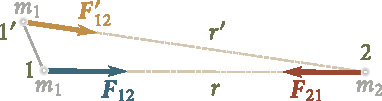
\includegraphics[scale=1]{figures/ch_02/fig_2_2.pdf}
		\caption[]{}
		\label{fig:2_2}
	\end{center}
\end{figure}

Ta hãy giả thử rằng lúc đầu các hạt $m_1$ và $m_2$ đứng yên tại các vị trí $1$ và $2$ (\fig{2_2}). Các lực tương tác $\vec{F}_{12}$ và $\vec{F}_{21}$ bằng nhau về độ lớn và ngược chiều nhau. Bây giờ giả thử hạt $m_1$ dịch chuyển rất nhanh (với vận tốc gần bằng $c$) tới vị trí $1'$. Tại điểm này trên hạt $m_1$ sẽ chịu tác dụng một lực $\vec{F}_{12}'$ nhỏ hơn về độ lớn ($r'>r$) và khác hướng so với $\vec{F}_{12}$ (ta hãy nhớ rằng trường của hạt $m_2$ vẫn không đổi). Còn lực $\vec{F}_{21}$ sẽ tiếp tục tác dụng lên hạt thứ hai, chừng nào mà sự nhiễu loạn của trường gây ra bởi sự dịch chuyển $m_1$ chưa đạt tới điểm $2$. Do đó chừng nào mà hạt $m_1$ đã chuyển động và trong suốt thời gian nào đó sau khi nó đã dừng lại ở điểm $1'$ thì định luật Newton thứ ba đã bị vi phạm.

Nếu hạt $m_1$ dịch chuyển từ điểm $1$ tới điểm $1'$ với vận tốc $v$ nhỏ hơn $c$ nhiều ($v\ll c$) và vận tốc truyền nhiễu loạn của trường đã lớn vô hạn thì các giá trị tức thời của trường ở điểm $2$ đã có thể đáp ứng cho các vị trí của hạt $m_1$ tại cùng thời điểm đó và do đó sự vi phạm định luật thứ ba đã không bị phát hiện.

Cơ học Newton nói chung chỉ đúng đối với các vận tốc chuyển động nhỏ hơn vận tốc ánh sáng nhiều (khi $v\ll c$). Do đó trong phạm vi của môn cơ học này vận tốc truyền nhiễu loạn của trường được coi là vô hạn, nên định luật Newton thứ ba luôn luôn được nghiệm đúng.

\section{Nguyên lý tương đối Galileo}\label{sec:2_7}

Ta hãy nghiên cứu hai hệ qui chiếu chuyển động đối với nhau với vận tốc không đổi $\vec{v}_0$. Một trong những hệ này được ký hiệu trên \fig{2_3} bằng chữ K, ta hãy coi nó một cách quy ước là hệ không chuyển động. Khi đó hệ thứ hai K$'$ sẽ chuyển động thẳng và đều. Ta hãy chọn các trục tọa độ $x, y, z$ của hệ K và các trục $x',y',z'$ của hệ K$'$ sao cho các trục x và $x'$ trùng nhau, còn các trục $y$ và $y'$ cũng như $z$ và $z'$ là song song với nhau.

\begin{figure}[!htb]
	\begin{center}
		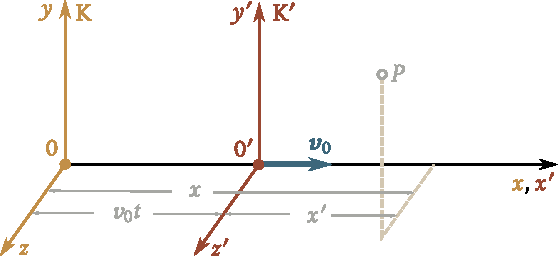
\includegraphics[scale=1]{figures/ch_02/fig_2_3.pdf}
		\caption[]{}
		\label{fig:2_3}
	\end{center}
\end{figure}

Ta hãy tìm sự liên hệ giữa các tọa độ $x, y, z$ của một điểm P nào đó trong hệ K và các tọa độ $x', y', z'$ cũng như điểm đó trong hệ K$'$. Nếu bắt đầu tính thời gian từ lúc mà các gốc tọa độ của hai hệ trùng nhau thì như suy ra từ \fig{2_3}, $x=x'+v_0t$. Ngoài ra, rõ ràng rằng $y=y'$ và $z=z'$. Sau khi đã bổ sung cho các hệ thức này một giả thuyết được thừa nhận trong cơ học cổ điển là thời gian trong cả hai hệ trôi như nhau, nghĩa là $t=t'$, ta được một tập hợp bốn phương trình
\begin{equation}\label{eq:2_19}
x=x'+v_0t,\quad y=y',\quad z=z',\quad t=t'.
\end{equation}

\noindent
gọi là \textbf{các phép biến đổi Galileo}.

Các hệ thức đầu và cuối của \eqref{eq:2_19} chỉ đúng với các giá trị $v_0$ nhỏ so với vận tốc ánh sáng trong chân không mà ta sẽ ký hiệu bằng chữ c $c$ ($v_0\ll c$). Khi $v_0$ vào cỡ $c$ các phép biến đổi Galileo phải được thay thế bằng các phép biến đổi Lorentz tổng quát hơn (xem Sec.~\ref{sec:8_2}). Trong phạm vi cơ học Newton, các công thức \eqref{eq:2_19} được coi là chính xác.

Lấy vi phân các hệ thức \eqref{eq:2_19} theo thời gian, ta hãy tìm sự liên hệ giữa các vận tốc của điểm P đối với các hệ quy chiếu K và K$'$:
\begin{align}
\dot{x} &= \dot{x}'+v_0, \quad\,\,\text{or}\quad\quad v_x=v_x'+v_0\nonumber\\
\dot{y} &= \dot{y}', \quad\quad\,\,\,\,\,\,\,\text{or}\quad\quad v_y=v_y'\label{eq:2_20}\\
\dot{z} &= \dot{z}', \quad\quad\,\,\,\,\,\,\,\,\text{or}\quad\quad v_z=v_z'.\nonumber
\end{align}

Ba hệ thức vô hướng \eqn{2_20} tương đương với hệ thức sau đây giữa vector vận tốc $\vec{v}$ đối với hệ K và vector vận tốc $\vec{v}'$ đối với hệ K$'$:
\begin{equation}\label{eq:2_21}
\vec{v} = \vec{v}' + \vec{v}_0.
\end{equation}

\noindent
Để thấy rõ điều này chỉ cần chiếu đẳng thức vector \eqref{eq:2_21} lên các trục $x, y, z$ là đủ. Kết quả là nguời ta được các công thức \eqref{eq:2_20}.

Các công thức \eqref{eq:2_20} và \eqref{eq:2_21} cho quy tắc cộng các vận tốc trong cơ học cổ điển. Cần để ý rằng hệ thức \eqn{2_21} cũng như mọi hệ thúc vector khác vẫn đúng khi chọn tùy ý các hướng tương hỗ của các trục tọa độ của các hệ K và K$'$. Còn các hệ thức \eqref{eq:2_20}, chỉ đúng khi chọn các trục đã chỉ trên \fig{2_3}.

Trong \ref{sec:2_2} ta đã chú ý rằng một hệ quy chiếu bất kỳ chuyển động đối với một hệ quán tính nào đó với vận tốc không đổi cũng sẽ là hệ quán tính. Bây giờ ta có khả năng chứng minh điều khẳng định này. Muốn vậy ta hãy lấy vi phân theo thời gian \eqn{2_21}. Nếu để ý rằng $\vec{v}_0$ là không đổi ta có
\begin{equation}\label{eq:2_22}
\dot{\vec{v}} = \dot{\vec{v}}', \quad\text{or}\quad  \vec{a} = \vec{a}'.
\end{equation}

\noindent
Từ đây suy ra rằng gia tốc của một vật bất kỳ, trong mọi hệ quy chiếu chuyển động thẳng và đều đối với nhau, là như nhau. Do đó nếu một trong những hệ này là hệ quán tính (điều này có nghĩa là khi không có các lực thì $\vec{a}=0$), thì các hệ còn lại cũng sẽ là các hệ quán tính ($\vec{a}'$ cũng bằng không).

Phương trình cơ bản của cơ học \eqref{eq:2_21} được đặc trưng bởi điều là, trong những đại lượng động học, nó chỉ chứa gia tốc, còn vạn tốc không tham gia vào trong đó. Tuy nhiên, như ta đã thiết lập ở trên, gia tốc của một vật bất kỳ trong hai hệ quy chiếu quán tính chọn tùy ý K và K$'$ là như nhau. Từ đó theo định luật Newton thứ hai suy ra rằng các lực tác dụng lên vật trong các hệ K và K$'$ cũng sẽ như nhau. Do đó, \textit{các phương trình động lực học không biến đổi khi chuyển từ hệ quy chiếu quán tính này sang hệ quy chiếu quán tính khác}, nghĩa là như người ta nói, là bất biến đổi đối với phép biến đổi tọa độ ứng với sự chuyển từ hệ quy chiếu quán tính này sang hệ quy chiếu quán tính khác. Theo quan điểm cơ học tất cả các hệ quy chiếu quán tính là hoàn toàn tương đương nhau: không nên ưu tiên hệ này hơn các hệ khác. Trong thực tế điều này thể hiện ở chỗ là không thể phát hiện hệ ở trạng thái nghỉ hay trạng thái chuyển động đều và thẳng bằng các thí nghiệm cơ học nào đã được biết trong phạm vi của hệ quy chiếu đã cho. Chẳng hạn, khi ngồi trong một toa tàu hỏa chuyển động thẳng và đều, không rung, và không nhìn qua cửa sổ ta không thể xác định được toa tàu chuyển động hay đứng yên. Sự rơi tự do của các vật, sự chuyển động của các vật do ta ném và mọi quá trình cơ học khác trong trường hợp này sẽ xảy ra như trong trường hợp nếu toa tàu không chuyển động.

Những sự kiện đã nêu còn được Galileo Galilei làm sáng tỏ. Luận điểm có nội dung là mọi hiện tượng cơ học trong những hệ quy chiếu quán tính khác nhau đều xảy ra một cách giống nhau, do đó không thể phát hiện được một hệ quy chiếu đã cho là đứng yên hay chuyển động thẳng và đều bằng các thí nghiệm cơ học nào, được gọi là \textbf{nguyên lý tương đối Galileo}.

\section{Các lực}\label{sec:2_8}

Trong vật lý hiện đại người ta phân biệt bốn dạng tương tác: (1) tương tác hấp dẫn (hoặc tương tác gây bởi sự hấp dẫn của vạn vật), (2) tương tác điện từ (được thực hiện thông qua các điện trường và từ trường), (3) tương tác mạnh hoặc tương tác hạt nhân (bảo đảm cho sự liên kết của các hạt trong hạt nhân nguyên tử), và (4) tương tác yếu (rất quan trọng trong nhiều quá trình phân rã các hạt cơ bản).

Trong phạm vi của cơ học cổ điển người ta đề cập đến các lực hấp dẫn và các lực điện từ cũng như các lực đàn hồi và các lực ma sát. Hai dạng lực cuối này được xác định bằng đặc trưng tương tác giữa các phân tử của các chất. Các lực tương tác giữa các phân tử có nguồn gốc điện từ. Do đó các lực đàn hồi và các lực ma sát về bản chất là các lực điện từ.

Các lực hấp dẫn và các lực điện từ là các lực cơ bản, không được quy chúng về các lực khác đơn giản hơn. Còn các lực đàn hồi và các lực ma sát không phải là các lực cơ bản.

Các định luật về các lực cơ bản là đặc biệt đơn giản. Độ lớn của lực hấp dẫn được xác định bằng \eqn{2_18}. Độ lớn của lực mà hai điện tích điểm đứng yên $q_1$ và $q_2$ tương tác với nhau được cho bởi định luật Coulomb:
\vspace{-12pt}
\begin{equation}\label{eq:2_23}
F = k\frac{q_1q_2}{r^2}
\end{equation}

\noindent
($k$ là hệ số tỷ lệ phụ thuộc vào việc chọn các đơn vị tham gia vào công thức của các đại lượng).

Nếu các điện tích chuyển động thì ngoài các lực \eqn{2_23} còn có các lực từ tác dụng lên chúng. Lực từ tác dụng lên một điện tích điểm $q$ chuyển động với vận tốc $\vec{v}$ trong từ trường có cảm ứng từ $\vec{B}$ được xác định bằng công thức
\begin{equation}\label{eq:2_24}
\vec{F} = k'q\,(\vecprod{v}{B})
\end{equation}

\noindent
($k'$ là hệ số tỷ lệ).

Các công thức \eqref{eq:2_18}, \eqref{eq:2_23} và \eqref{eq:2_24} là chính xác. Đối với các lực đàn hồi và các lực ma sát có thể chỉ thu được các công thức thực nghiệm gần đúng mà chúng ta sẽ nghiên cứu trong các mục sau.

\section{Các lực đàn hồi}\label{sec:2_9}

Dưới tác dụng của những lực đặt lên nó, mọi vật thực sẽ bị biến dạng, nghĩa là biến đổi kích thước và hình dạng của mình. Nếu sau khi ngừng tác dụng các lực, vật lại nhận các kích thước và hình dạng ban đầu thì sự biến dạng được gọi là \textbf{sự biến dạng đàn hồi}. Các biến dạng đàn hồi được quan sát trong trường hợp nếu lực gây ra biến dạng không vượt quá một giới hạn nào đó (giới hạn đàn hổi) được xác định cho mỗi vật cụ thể.

\begin{figure}[!htb]
	\begin{center}
		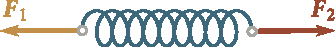
\includegraphics[scale=1]{figures/ch_02/fig_2_4.pdf}
		\caption[]{}
		\label{fig:2_4}
	\end{center}
\end{figure}

Ta hãy lấy một lò xo có độ dài $l_0$ ở trạng thái không biến dạng và đặt ở đầu lò xo những lực $\vec{F}_1$ và $\vec{F}_2$ bằng nhau về độ lớn và ngược chiều nhau (\fig{2_4}). Dưới tác dụng của các lực này, lò xo bị kéo căng ra một lương $\Delta l$ nào đó, sau đó sự cân bằng lại xảy ra. Ở trạng thái cân bằng các ngoại lực $\vec{F}_1$ và $\vec{F}_2$ sẽ được cân bằng bởi các lực đàn hồi sinh ra trong lò xo do biến dạng. Thí nghiệm cho rằng, với các biến dạng không lớn độ dãn $\Delta l$ của lò xo tỷ lệ với lực kéo căng: $\Delta l\propto F$ (here $F=F_1=F_2$). Một cách tương ứng, lực đàn hồi tỷ lệ với độ dãn của lò xo:
\begin{equation}\label{eq:2_25}
F = k\,\Delta l.
\end{equation}

\noindent
Hệ số tỷ lệ k được gọi là \textbf{hệ số độ cứng} của lò xo.

Điều khẳng định về sự tỷ lệ giữa lực đàn hồi và sự biến dạng được gọi là \textbf{định luật Hooke}.

Các sự dãn đàn hồi xuất hiện trong mọi lò xo. Một phần bất kỳ của lò xo tác dụng lên một phần khác một lực xác định bằng \eqn{2_25}. Do đó nếu cắt lò xo làm đôi thì sẽ xuất hiện một lực đàn hồi có cùng độ lớn trong mỗi nửa với độ dãn nhỏ hơn hai lần. Từ đó ta kết luận rằng với vật liệu đã cho của lò xò và với các kích thước đã cho của vòng xoắn, độ lớn của lực đàn hồi được xác định không phải bằng độ dãn tuyệt đối $\Delta l$ của lò xo mà bằng độ dãn tỷ đối $\Delta l/l_0$.

Khi nén lò xo, cũng xuất hiện các lực căng đàn hồi nhưng có dấu khác. Ta hãy tổng quát hóa \eqn{2_25} bằng cách sau. Đóng chặt đầu này của lò xo (\fig{2_5}) và sẽ coi độ dãn của lò xo như tọa độ $x$ của đầu kia, tính từ vị trí của nó ứng với lò xo không bị biến dạng\footnote{Trên\fig{2_5}b, độ dài đoạn dịch chuyển của đầu lo xo được ký hiệu là $-x$, đó là độ dài của một đoạn thẳng là một đại lượng dương còn tọa độ $x$ trong trường hợp này là âm.}. Ngoài ra, ta sẽ hiểu $F$ là hình chiếu lên trục $x$ của $\vec{F}_{\text{el}}$. Khi đó có thể viết là
\begin{equation}\label{eq:2_26}
F = -k x
\end{equation}

(từ \fig{2_5} rõ ràng là hình chiếu của lực đàn hồi lên trục $x$ và tọa độ $x$ luôn luôn có các dấu khác nhau).

\begin{figure}[!htb]
	\begin{minipage}[t]{0.5\linewidth}
		\begin{center}
			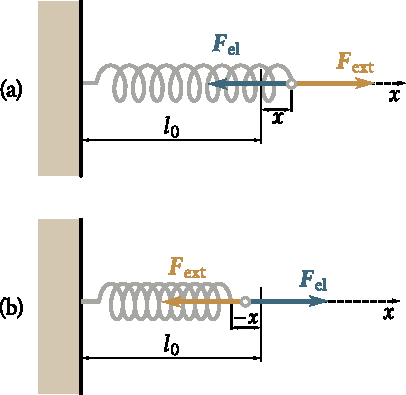
\includegraphics[scale=0.75]{figures/ch_02/fig_2_5.pdf}
			\caption[]{}
			\label{fig:2_5}
		\end{center}
	\end{minipage}
	\hspace{-0.05cm}
	\begin{minipage}[t]{0.5\linewidth}
		\begin{center}
			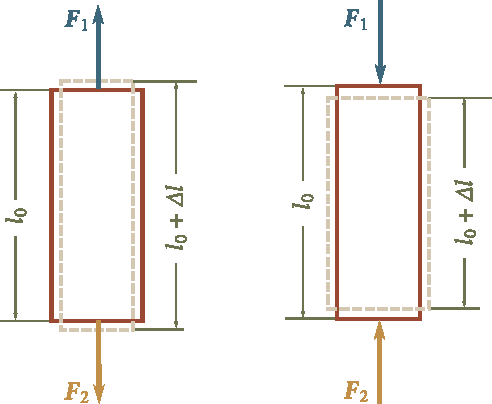
\includegraphics[scale=0.70]{figures/ch_02/fig_2_6.pdf}
			\caption[]{}
			\label{fig:2_6}
		\end{center}
	\end{minipage}
\end{figure}

Các thanh đồng chất có đặc tính giống như lò xo khi dãn hoặc khi nén theo một phía. Nếu tại các đàu của thanh đặt các lực $\vec{F}_1$ và $\vec{F}_2$ ($F_1=F_2=F$) hướng dọc theo trục của nó mà tác dụng của chúng được phân bố đều theo toàn tiết diện, thì độ dài $l_0$ của thanh nhận số gia\footnote{Sự biến đổi độ dài của thanh kéo theo sự biến đổi tương ứng các tiết diện ngang của thanh.} $\Delta l$ dương (khi dãn) hoặc âm (khi nén) (\fig{2_6}). Để làm địa lượng đặc trưng cho sự biến dạng của thanh, người ta lấy một cách tự nhiên độ biến thiên tỷ đối của độ dài của nó:
\begin{equation}\label{eq:2_27}
\varepsilon = \frac{\Delta l}{l_0}.
\end{equation}

Thí nghiệm chứng tỏ rằng đối với các thanh làm bằng vật liệu đã cho độ dãn tỷ đối khi biến dạng đàn hồi tỷ lệ với lực dược tính cho một đơn vị diện tích tiết diện ngang của thanh:
\begin{equation}\label{eq:2_28}
\varepsilon = \alpha\frac{\Delta l}{S}.
\end{equation}

\noindent
($\alpha$ là hệ số tỷ lệ).

Đại lượng bằng tỷ số giữa lực với độ lớn của bề mặt mà trên đó lực tác dụng được gọi là \textbf{ứng suất}. Do tương tác của các phần của vật với nhau, ứng suất được truyền cho tất cả các điểm của vật, nghĩa là toàn bộ thể tích của thanh ở trong trạng thái chịu ứng lực. Nếu lực hướng theo pháp tuyến của mặt thì ứng suất được gọi là \textbf{ứng suất pháp tuyến}. Nếu lực hướng theo tiếp tuyến với mặt mà nó tác dụng thì ứng suất được gọi là \textbf{ứng suất tiếp tuyến}. Ứng suất pháp tuyến thường được ký hiệu bằng chữ $\sigma$, ứng suất tiếp tuyến bằng chữ $\tau$.

Tỷ số $F/S$ trong \eqn{2_28} là ứng suất pháp tuyến $\sigma$. Do đó có thể cho công thức này dạng:
\begin{equation}\label{eq:2_29}
\varepsilon = \alpha\sigma.
\end{equation}

\noindent
Để đặc trưng cho các tính chất đàn hồi của vật liệu người ta dùng đại lượng $E=1/\alpha$ được gọi là \textbf{suất Young. Đại lượng này được đo bằng pascal} ($\SI{1}{\pascal}=\SI{1}{\newton\per\square\metre}$).

Thay thế $\alpha$ trong \eqn{2_9} bằng $1/E$, ta có được hệ thức:
\begin{equation}\label{eq:2_30}
\varepsilon = \frac{\alpha}{E}
\end{equation}

\noindent
từ đó suy ra rằng suất Young sẽ bằng ứng suất pháp tuyến khi độ dãn tỷ đối đã bằng đơn vị (tức là số gia của độ dài $\Delta l$ đã bằng độ dài $l_0$ ban đầu), nếu các biến dạng đàn hồi hết sức lớn đã xảy ra (trong thực tế sự phá hủy thanh xảy ra với các ứng suất nhỏ hơn rất nhiều nên giới hạn đàn đồi đã đạt được sớm hơn).

Giải \eqn{2_28} đối với $F$ và thay thế $\varepsilon$ bằng $\Delta l/l_0$ còn $\alpha$ bằng $1/E$ ta được công thức
\begin{equation}\label{eq:2_31}
F = \frac{E\,S}{l_0}\Delta l = k\,\Delta l
\end{equation}

\noindent
trong đó $k$ là hệ số không đôi đối với thanh đã cho. Hệ thức \eqref{eq:2_31} biểu thị định luật Hooke cho một thanh [so sánh với \eqn{2_26}]. Ta nhớ rằng định luật này chỉ nghiệm đúng khi giới hạn đàn hồi chưa đạt được

\begin{figure}[!htb]
	\begin{center}
		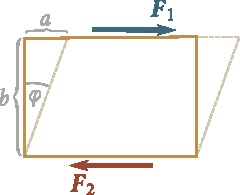
\includegraphics[scale=1]{figures/ch_02/fig_2_7.pdf}
		\caption[]{}
		\label{fig:2_7}
	\end{center}
\end{figure}

Cuối cùng ta hãy nghiên cứu ngắn gọn sự biến dạng dịch. Lấy một vật đồng chất có dạng hình hộp chữ nhật và đặt vào các mặt đối diện của nó các lực $\vec{F}_1$ và $\vec{F}_2$ ($F_1=F_2=F$) hướng song song với các mặt này (~\fig{2_7}). Nếu tác dụng của các lực được phân bố đều theo tất cả bề mặt của mặt tương ứng thì tại một tiết diện bất kỳ song song với các mặt này sẽ xuất hiện một ứng suất tiếp tuyến
\begin{equation}\label{eq:2_32}
\tau = \frac{F}{S}
\end{equation}

\noindent
($S$ là diện tích của mặt). Dưới tác dụng của ứng suất vật bị biến sạng sao cho mặt này bị dịch đối với mặt kia một khoảng $a$ nào đó. Nếu chia vật một cách tưởng tượng thành các lớp mỏng song song với các mặt được khảo sát thì mỗi lớp được dịch đi so với các lớp ở bên cạnh nó. Do nguyên nhân này sự biến dạng có dạng như thế được gọi là \textbf{sự biến dạng dịch}.

Với biến dạng dịch một đường thẳng bất kỳ lúc đầu vuông góc với các lớp sẽ quay đi một góc $\varphi$ nào đó. Để đặc trưng cho biến dạng dịch người ta lấy đại lượng
\begin{equation}\label{eq:2_33}
\gamma = \frac{a}{b} = \tan\varphi
\end{equation}

\noindent
được gọi là \textbf{độ dịch tỷ đối} (ý nghĩa của địa lượng $a$ và $b$ được minh họa trên \fig{2_7}). Với các biến dạng đàn hồi, góc $\varphi$ là rất nhỏ. Vì vật có thể đặt $\tan\varphi\approx\varphi$. Do đó độ dịch tỷ đối bằng góc dịch $\varphi$.

Thí nghiệm chứng tỏ rằng độ dịch tỷ đối tỷ lệ với ứng suất tiếp tuyến
\vspace{-12pt}
\begin{equation}\label{eq:2_34}
\gamma = \frac{1}{G}\tau.
\end{equation}

\noindent
Hệ số $G$ chỉ phụ thuộc vào các tính chất của vật liệu và được gọi là \textbf{suất trượt}. Nó sẽ bằng ứng suất tiếp tuyến khi góc dịch bằng 45 độ ($\tan\varphi=1$), nếu như các biến dạng rất lớn giới hạn đàn hồi đã không bị vượt quá. $G$ và cả $E$ đều được đo bằng (\si{\pascal}).

\section{Các lực ma sát}\label{sec:2_10}

Các lực ma sát xuất hiện trong sự dịch chuyển các vật tiếp xúc với nhau hoặc các phần của chúng đối với nhau. Sự ma sát sinh ra trong sự dịch chuyển tương đối giữa hai vật tiếp xúc với nhau được gọi là \textbf{sự ma sát ngoài}; sự ma sát giữa các phần của cùng một vật liên tục (chẳng hạn, của chất lỏng hoặc chất khí) được gọi là \textbf{sự ma sát trong}.

Cần phải xếp lực ma sát xuất hiện khi một vật rắn chuyển động trong môi trường lỏng hay khí vào loại các lực nội ma sát, vì trong trường hợp này các lớp môi trường trực tiếp tiếp xúc với vật bị lôi kéo vào chuyển động với cùng một vận tốc mà vật có, và sự ma sát giã các lớp này và các lớp môi trường ở bên ngoài đối với chúng sẽ ảnh hưởng tới sự chuyển động của vật.

Sự ma sát giữa các bề mặt của hai vật rắn khi không có một lớp giữa nào đó, chẳng hạn không có sự bôi trơn giữa chúng, được gọi là \textbf{sự ma sát khô}. Sự ma sát giữa một vật rắn và một môi trường lỏng hay khí, cũng như giữa các lớp của môi trường đó được gọi là \textbf{sự ma sát nhớt} (hoặc \textbf{sự ma sát lỏng}).

Đối với sự ma sát khô người ta phân biệt: \textbf{sự ma sát trượt} và \textbf{sự ma sát lăn}.

Các lực ma sát hướng theo tiếp tuyến các mặt trượt (hoặc các lớp), đồng thời sao cho chúng chống lại sự dịch chuyển tương đối của các mặt (các lớp) này. Chẳng hạn, nếu hai lớp chất lỏng trượt lên nhau, chuyển động với vận tốc khác nhau thì lực đặt vào lớp chuyển động nhanh hơn hướng về phía ngược với chuyển động, còn lực tác dụng lên lớp cuyển động chậm hơn hướng về phía chuyển động của lớp này.

\begin{figure}[!htb]
	\begin{center}
		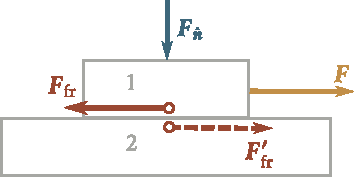
\includegraphics[scale=1]{figures/ch_02/fig_2_8.pdf}
		\caption[]{}
		\label{fig:2_8}
	\end{center}
\end{figure}

\textbf{Sự ma sát khô.} Trong trường hợp ma sát khô lực ma sát xuất hiện không chỉ khi một mặt này trượt trên mặt kia mà cũng cả khi định gây ra sự trượt như thế. Ta hãy xét hai vật $1$ và $2$ tiếp xúc nhau trong đó vật $2$ cố định (\fig{2_8}). Vật $1$ được ép vào vật $2$ bằng lực $\vec{F}_{\hatvec{n}}$ hướng theo pháp tuyến của mặt tiếp xúc của các vật. Nó được gọi là \textbf{áp lực pháp tuyến} và có thể được gây bởi trọng lượng của vật hoặc bởi các nguyên nhân khác. Ta thử dịch chuyển vật $1$ bằng cách tác dụng lên vật một ngoại lực $\vec{F}$. Khi đó người ta phát hiện rằng đối với mỗi cặp vật cụ thể và mỗi giá trị của áp lực pháp tuyến có một giá trị cực tiểu xác định $F_0$ của lực $\vec{F}$ làm cho vật $1$ chuyển dịch được. Với các giá trị của ngoại lực nằm trong các giới hạn từ $0$ đến $F_0$, vật vẫn còn đứng yên. Theo định luật Newton thứ hai, điều này có thể xảy ra trong trường hợp nếu lực $\vec{F}$ được cân bằng với một lực bằng nó về độ lớn nhưng ngược chiều; lực này là lực ma sát nghỉ $\vec{F}_{\text{fr}}$ (xem~\fig{2_8}). Nó tự động\footnote{Điều này xảy ra tương tự như dưới tác dụng của các lực kéo, một lò xo tự động có một độ dãn mà với độ dãn này lực đàn hồi cân bằng với ngoại lực.} nhận giá trị bằng độ lớn $F$ (với điều kiện là lực này không vượt quá $F_0$). Đại lượng $F_0$ là giá trị lớn nhất của lực ma sát nghỉ.

Ta hãy chú ý rằng ứng với định luật Newton thứ ba trên vật $2$ cũng có lực ma sát nghỉ $\vec{F}_{\text{fr}}'$ (trên \fig{2_8}) nó được vẽ bằng đường chấm chấm), bằng lực $\vec{F}_{\text{fr}}$ về độ lớn nhưng có chiều ngược với nó.

Nếu ngoại lực $\vec{F}$ trội hơn $F_0$ về module, thì vật bắt đầu trượt đồng thời gia tốc của vật được xác định bằng hợp lực của hai lực: ngoại lực $\vec{F}$ và lực ma sát nghỉ $\vec{F}_{\text{fr}}$, có độ lớn ở mức nào đó phụ thuộc vào vận tốc trượt. Đặc trưng của sự phục thuộc này được xác định bằng bản chất và trạng thái của các bề mặt trượt. Dạng phụ thuộc của lực ma sát vào vận tốc thường gặp nhất được trình bày trên \fig{2_9}. Đồ thị bao gồm cả trường hợp nghỉ và cả trường hợp trượt. Lực ma sát nghỉ, như đã chỉ rõ, có thể có giát rị từ $0$ đến $F_0$ và được phản ahr trên đồ thị bằng đonạ thẳng đứng. Theo \fig{2_9}, với sự tăng của vận tốc, lực ma sát trượt lúc đầu giảm đi một ít và sau đó lại bắt đầu tăng.
Với sự gia công đặc biệt các mặt tiếp xúc với nhau lực ma sát trượt trên thực tế có thể không phụ thuộc vào vận tốc. Trong trường hợp này phần cong của đọ thi trên \fig{2_9} trở thành đoạn thẳng nằm ngang bắt đầu tại điểm $F_0$.

\begin{figure}[!htb]
	\begin{center}
		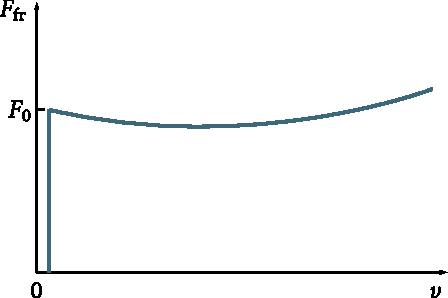
\includegraphics[scale=0.98]{figures/ch_02/fig_2_9.pdf}
		\caption[]{}
		\label{fig:2_9}
	\end{center}
\end{figure}

Các định luật về ma sát khô được quy lại như sau: lực ma sát nghỉ cực đại, cũng như lực ma sát trượt, không phụ thuộc vào diện tích tiếp xúc của các vật trượt và tỷ lệ gần đúng với độ lớn của áp lực pháp tuyến ép các mặt trượt với nhau:
\begin{equation}\label{eq:2_35}
F_{\text{fr}} = f\,F_{\hatvec{n}}.
\end{equation}

\noindent
Hệ số tỷ lệ $f$ không có thú nguyên được gọi là \textbf{hệ số ma sát trượt} (ứng với ma sát nghỉ hay ma sát trượt). Nó phụ thuộc vào bản chất và trạng thái của các mặt trượt, đặc biệt vào độ nhám của chúng. Trong trường hợp trượt, hệ số ma sát là hàm của vận tốc.

Các lực ma sát đóng vai trò rất lớn trong tự nhiên. Trong đời sống hàng ngày của chúng ta sự ma sát luôn luôn có ích. Ta hãy nhớ lại những nỗi khó khăn lớn mà những người đi bộ và các phương tiện vận tải phải trải qua trong thời gian băng phủ mặt đường, khi mà sự ma sát giữa chất phủ lên mặt đường và các đế giày của những người đi bộ hoặc các bánh xe của phương tiện vận tải bị giảm đáng kể. Không có các lực ma sát, thì như trên tàu thủy trong lúc chòng chành, đồ gỗ cần phải gắn chặt vào sàn vì với sự không nằm ngang nhỏ nhất của sàn, nó tụt theo hướng dốc thoai thoải. Bạn đọc có thể tự tìm các vị dú tương tự

Trong nhiều trường hợp vai trò của lực ma sát rất có hại, và cần phải áp dụng biện pháp làm yếu nó tới mức có thể được. Chẳng hạn, tình hình xyar ra với sự ma sát ở trong các ổ bi hoặc có sự ma sát giữa ô trục của bánh xe và trục.

Cách làm giảm cơ bản nhất các lực ma sát là thay thế ma sát trượt bằng sự ma sát lăn, xuất hiện, chẳng hạn, giữa một vật hình trụ hoặc hình cầu và một mặt cong theo đó vật lăn. Sự ma sát lăn về hình thức tuân theo cùng các quy luật như sự ma sát trượt nhưng hệ số ma sát trong trường hợp này là rất nhỏ.

\textbf{Sự ma sát nhớt và sự cản trở của môi trường.} Khác với sự ma sát khô, sự ma sát nhớt được đặc trưng bởi điều là lực ma sát nhớt triệt tiêu đồng thời với vận tốc. Do đó một ngoại lực nhỏ như thế nào đi nữa cũng có thể tăng thêm vận tốc tương đối cho các lớp của môi trường nhớt. Các định luật mà lực ma sát giữa các lớp của môi trường phải tuân theo sẽ được nghiên cứu trong chương dành cho cơ học các chất lỏng.

\begin{figure}[!htb]
	\begin{center}
		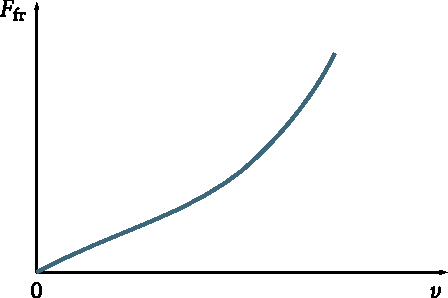
\includegraphics[scale=1]{figures/ch_02/fig_2_10.pdf}
		\caption[]{}
		\label{fig:2_10}
	\end{center}
\end{figure}

Trong tiết này, chúng tôi hạn chế ở việc nghiên cứu các lực ma sát giữa vật rắn và môi trường nhớt (môi trường lỏng hoặc khí). Cần chú ý rằng, thực ra ngoài các lực ma sát, khi các vật chuyển động trong môi trường lỏng hoặc khí, còn xuất hiện các lực cản của môi trường; chúng có thể lớn hơn các lực ma sát rất nhiều. Nếu không có khả năng nghiên cứu tỉ mỉ các nguyên nhân sinh ra các lực này thì ta giới hạn ở sự trình bày các tính quy luật mà các lực ma sát và các lực cản của mô itruowfng cùng tuân theo, đồng thời ta sẽ gọi một cách quy ước lực tổng hợp là lực ma sát. Sự phụ thuộc của các lực này vào vận tốc được trình bày trên \fig{2_10}.

Với các vận tốc không lớn, lực tăng tuyến tính với vận tốc:
\begin{equation}\label{eq:2_36}
\vec{F}_{\text{fr}} = -k_1 \vec{v}
\end{equation}

\noindent
(dấu trừ có nghĩa là lực này hướng ngược chiều với vận tốc). Độ lớn của hệ số $k_1$ phụ thuộc vào dạng và các kích thước của vật, trạng thái bề mặt của nó và vào tính chất của môi trường được gọi là độ nhớt. Chẳng hạn, đối với glycerin hệ số này lớn hơn đối với nước rất nhiều.

Với các vận tốc lớn, định luật tuyến tính chuyển thành định luật bình phương, tức là lực bắt đầu tăng tỷ lệ với bình phương của vận tốc:
\begin{equation}\label{eq:2_37}
\vec{F}_{\text{fr}} = -k_2\, v^2\, \vecuni{v}
\end{equation}

\noindent
($\vecuni{v}$ là chuẩn của vận tốc). Độ lớn của hệ số $k_2$ phụ thuộc vào các kích thước và hình dạng của vật.

Giá trị của vận tốc tại đó định luật \eqref{eq:2_36} chuyển thành \eqref{eq:2_37} sẽ phụ thuộc vào hình dạng và kích thước của vật cũng như phụ thuộc vào các tính chất nhớt và khối lượng riêng của môi trường.

\section{Trọng lực và trọng lượng}\label{sec:2_11}

Dưới tác dụng của lực hút về Trái đất mọi vật rơi với một gia tốc đối với mặt đất được ký hiệu bằng chữ $g$. Điều này có nghĩa là trong hệ quy chiếu gắn với Trái đất, mỗi vật có khối lượng $m$ chịu tác dụng một lực
\begin{equation}\label{eq:2_38}
\vec{P} = m\vec{g}
\end{equation}

\noindent
được gọi là trọng lực\footnote{Do tính không quán tính của hệ quy chiếu gắn với Trái đất, trọng lực khác ít so với lực mà vật bị trái đất hút. Chi tiết về điều này sẽ nói trong \ref{sec:4_2}.}. Khi vật đứng yên đối với mặt đất thì lực $\vec{P}$ được cân bằng bởi phản lực\footnote{Các lực mà các vật tác dụng lên vật đã cho, làm hạn chế sự chuyển động của nó, được gọi là các phản lực.} $\vec{F}_{\text{r}}$ của giá treo hoặc giá đỡ giữ cho vật khỏi rơi ($\vec{F}_{\text{r}}=-\vec{P}$). Theo định luật Newton thứ ba trong trường hợp này vật tác dụng lên giá treo hoặc giá đỡ một lực $\vec{W}$ bằng $-\vec{F}_{\text{r}}$, tức là một lực
\begin{equation*}
\vec{W} = \vec{P} = m\vec{g}
\end{equation*}

\begin{figure}[!htb]
	\begin{center}
		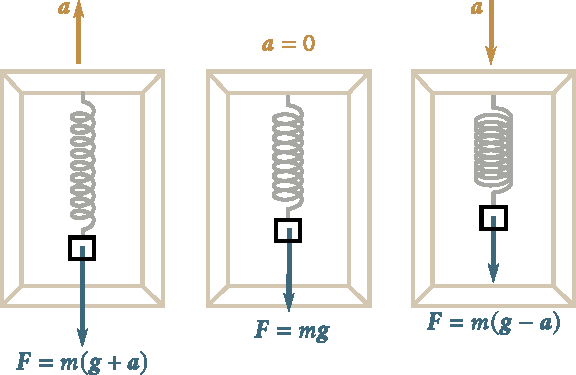
\includegraphics[scale=1]{figures/ch_02/fig_2_11.pdf}
		\caption[]{}
		\label{fig:2_11}
	\end{center}
\end{figure}

Lực $\vec{W}$ mà vật tác dụng lên giá treo hoặc giá đỡ được gọi là \textbf{trọng lượng} của vật. Lực này bằng $m\vec{g}$ chỉ trong trường hợp nếu vật và giá đỡ (hoặc giá treo) không chuyển động đối với Trái đất. Trong trường hợp chúng chuyển động với một gia tốc $\vec{a}$ nào đó, trọng lượng $\vec{W}$ sẽ không bằng $m\vec{g}$. Có thể làm sáng tỏ điều này bằng ví dụ sau đây. Giả thử giá treo là một lò xo được đóng chặt vào một cái khung và chuyển động cùng với vật với gia tốc $\vec{a}$ (\fig{2_11}). Khi đó phương trình chuyển động của vật sẽ có dạng
\begin{equation}\label{eq:2_39}
\vec{P} + \vec{F}_{\text{r}} = m\vec{a}
\end{equation}

\noindent
trong đó $\vec{F}_{\text{r}}$ là phản lực của giá treo, tức là lực mà lò xò tác dụng lên vật. Theo định luật Newton thứ ba vật tác dụng lên lò xo một bằng bằng $-\vec{F}_{\text{r}}$ mà theo định nghĩa là trong lượng $\vec{W}$ của vật trong các điều kiện này. Thay thế phản lực $\vec{F}_{\text{r}}$ trong \eqn{2_39} bằng lực $-\vec{W}$, còn trọng lực $\vec{P}$ bằng tích số $m\vec{g}$, ta được
\begin{equation}\label{eq:2_40}
\vec{W} = m(\vec{g} - \vec{a}).
\end{equation}

\noindent
Công thức \eqref{eq:2_40} xác định trọng lượng của vật trong trường hợp tổng quát. Nó đúng đối với giá treo hoặc giá đỡ có dạng bất kỳ.
Ta giả thử rằng vật và giá treo chuyển động theo hướng thẳng đứng (\fig{2_11} ứng với giả thiết này).

Ta chiếu \eqn{2_40} lên hướng của dây rọi:
\begin{equation}\label{eq:2_41}
W = m(g \pm a).
\end{equation}

\noindent
Trong biểu thức này, $W$, $g$, và $a$ là module của các vector tương ứng. Dấu "+" ứng với a hướng lên trên, dấu "-" ứng với hướng của a xuống dưới.

Từ \eqn{2_41}, suy ra rằng, về module trọng trường $\vec{W}$ có thể lớn hơn hoặc nhỏ hơn trọng lực $\vec{P}$. Khi khung với giá treo rơi tự do thì, $\vec{a}=\vec{g}$, và lực $\vec{W}$ mà vật tác dụng lên giá treo bằng không. Trạng thái không trọng lượng bắt đầu. Con tàu vũ trụ bay xung quanh Trái đất với các động cơ bị tắt sẽ chuyển động như một khung rơi tự do với gia tốc $\vec{g}$, vì vậy các vật trong con tàu ở trạng thái không trọng lượng, nghĩa là chúng không gây áp suất lên các vật tiếp xúc với chúng.

Ta hãy để ý rằng, thường người ta hay nhầm lẫn trọng lực $\vec{P}$ và trọng lượng $\vec{W}$ của vật. Điều này xảy ra là do trong trường hợp giá đỡ không chuyển động các lực $\vec{P}$ và $\vec{P}$ trùng nhau về độ lớn và hướng (cả hai đều bằng $m\vec{g}$). Tuy nhiên cần phải nhớ rằng các lực này được đặt vào các vật khác nhau: $\vec{P}$ được đặt vào chính vật, $\vec{W}$ được đặt vào giá treo hoặc giá đỡ, hạn chế chuyển động tự do của vật trong trường lực hút của Trái đất. Ngoài ra, lực $\vec{P}$ luôn luôn bằng $m\vec{g}$, không phụ thuộc vào vật chuyển động hay đứng yên, còn lực của trọng lượng $\vec{W}$ phụ thuộc vào gia tốc của giá đỡ và vật chuyển động, thêm vào đó nó có thể hoặc lớn hơn hoặc nhỏ hơn $m\vec{g}$ và đặc biệt là nó triệt tiêu ở trạng thái không trọng lượng.

Hệ thức \eqref{eq:2_40} giữa khối lượng và trọng lượng của vật cho cách so sánh các khối lượng của các vật bằng cách cân: tỷ số các trọng lượng của các vật được xác định trong những điều kiện giống nhau (thông thường với $\vec{a}=0$) tại cùng một điểm trên mặt đất bằng tỷ số các khối lượng của các vật này:
\begin{equation*}
W_1\,:\,W_2\,:\,W_3\,:\,\ldots = m_1\,:\,m_2\,:\,m_3\ldots.
\end{equation*}

Như sẽ chứng tỏ trong \ref{sec:4_2}, gia tốc rơi tự do $g$ và trọng lực $P$ phụ thuộc vào vĩ độ của khu vực. Ngoài ra, $P$ và $g$ cũng phụ thuộc vào độ cao trên mặt biển - chúng sẽ giảm khi đi ra xa tâm Trái đất.

\section{Ứng dụng thực tế của các định luật Newton}\label{sec:2_12}

\begin{figure}[!htb]
	\begin{center}
		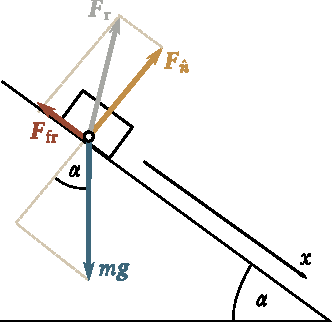
\includegraphics[scale=1]{figures/ch_02/fig_2_12.pdf}
		\caption[]{}
		\label{fig:2_12}
	\end{center}
\end{figure}

Để thành lập phương trình chuyển động trước hết cần phải thiết lập những lực nào tác dụng lên vật đang khảo sát. Đồng thời cần chú ý làm sáng tỏ tác dụng của các vật nào khác lên vật đã cho. Chẳng hạn đối với vật trượt trên mặt phẳng nghiêng (\fig{2_12}), thì tác động từ phía Trái đất (được đặc trưng bằng lực $m\vec{g}$) và tác động từ phía mặt phẳng (được đặc trưng bằng phản lực $\vec{F}_{\text{r}}$) là chủ yếu.

Hoàn toàn không cần đưa vào sự khảo sát các lực ``chuyển động'', ``lăn'', ``hướng tâm'', ``ly tâm''\footnote{Điều này không liên quan tới thuật ngữ ``lực quán tính ly tâm'' (xem Sec.~\ref{sec:4_2}.} và các lực tương tự như thế. Để tránh sai lầm cần phải đặc trưng các lực không theo tác dụng do chúng gây ra mà theo ``nguồn gốc'' gây ra sự xuất hiện lực. Điều này có nghĩa là ứng với mỗi lực cần phải nhìn thấy vật mà lực được gây ra bởi sự tác động của vật. Khi đó rõ ràng sẽ không thể xảy ra sai sót điển hình là cùng một lực được hai lần tính đến dưới các tên gọi khác nhau.

Trong ví dụ đang xét (xem~\fig{2_12}), một cách hợp lý là chia phản lực $\vec{F}_{\text{r}}$ thành hai phần là lực pháp tuyến $\vec{F}_{\hatvec{n}}$ và lực ma sát $\vec{F}_{\text{fr}}$. Đặc biệt điều này có lợi vì lực ma sát tỷ lệ mới module của lực $\vec{F}_{\hatvec{n}}$ [xem~\eqn{2_35}].

Sau khi xác định các lực tác dụng lên vật người ta thành lập phương trình của định luật Newton thứ hai. Trong ví dụ của ta nó có dạng
\begin{equation}\label{eq:2_42}
m\vec{a} = m\vec{g} + \vec{F}_{\text{r}} = m\vec{g} + \vec{F}_{\hatvec{n}} + \vec{F}_{\text{fr}}.
\end{equation}

\noindent
Để thực hiện các phép tính toán cần phải chuyển từ các vector sang các hình chiếu của chúng lên các hướng đã chọn một cách thích hợp. Đồng thời người ta sử dụng các tính chất sau đây của hình chiếu:
\begin{enumerate}[(1)]
	\item các vector bằng nhau có các hình chiếu như nhau;
	\item hình chiếu của vector mà vector này bằng tích của một vector khác với một vô hướng, sẽ bằng tích hình chiếu của vector thứ hai này với vô hướng đó;
	\item hình chiếu của tổng các vector bằng tổng các hình chiếu của các vector số hạng [xem~\eqn{1_8}].
\end{enumerate}

Ta hãy chiếu các vector tham gia vào \eqn{2_42} lên hướng $x$ đã nêu trên \fig{2_12}. Hình chiếu của các vector bằng $a_x=a$ ($a$ là module của vector $\vec{a}$), $g_x=g\sin\alpha$, $F_{\hatvec{n}x}=0$, $F_{\text{r}x}=-f F_{\hatvec{n}x}=-fmg\cos\alpha$. Do đó ta đi đến phương trình
\begin{equation*}
ma = mg\sin\alpha - fmg\cos\alpha
\end{equation*}

\noindent
mà từ phương trình này dễ dàng tìm được $a$.

Trong các trường hợp phức tạp hơn đành phải chiếu các vector lên một số hướng và giải hệ các phương trình đại số hoặc vi phân thu được.
